% PREAMBLE + START -
\documentclass[12pt]{article}

\usepackage[]{microtype}
\usepackage[margin=0.21in]{geometry}
\usepackage{amsmath,amsfonts,mathtools,hyperref,graphicx,amssymb,bm}
\hypersetup{colorlinks=true}
\graphicspath{{./3-img/}}

% padded box (answers)
\newcommand{\paddedBox}[1]{{\setlength\fboxsep{5pt}\boxed{#1}}}
% binomial exponent
\newcommand{\negativeBinomial}[3][2]{(#2- #3)^{#1}}
% large math
\newcommand*{\largeMath}[1]{\mbox{\Large$#1$}}
% huge math
\newcommand*{\hugeMath}[1]{\mbox{\huge$#1$}}

\begin{document}

% SECTION: RMSD: Root-Mean-Square-Deviation: -
\section*{Root-Mean-Square-Deviation/Error (RMSD/RMSE)}

\paragraph{}
	The \textbf{root-mean-square-deviation (RMSD)} or \textbf{root-mean-square-error (RMSE)} is a frequently used measure of the differences between values (sample or population) predicted by a model or an \textbf{estimator} and the values observed. It represents the square root of the second \textbf{sample moment} of the differences between predicted values and observed values or the \textbf{quadratic mean} of these differences. These \textbf{deviations} are called \textbf{residuals} when the calculations are preformed over the data sample that was used for estimation and are called \emph{errors} (or prediction errors) when computed out-of-sample.

\paragraph{Data:}

\begin{align*} % three column align
	\text{actual: }(x, y) && \text{predicted: } & (x, y) &&
	\mathbf{\bar{x}} = 2 & \mathbf{\bar{y}} & = 3 \\
	(1, 1) && & (1, 0.5) && \mathbf{s_{x}} = 0.816 & \mathbf{s_{y}} & = 2.160 \\
	(2, 2) && & (2, 3) \\
	(2, 3) && & (2, 3) \\
	(3, 6) && & (3, 5.5) && (\text{Prediction Formula: }\hat{y} = 2.50x - 2)
\end{align*}

\paragraph{Insight:}
The \textbf{i\textsuperscript{th}} residual will be equal to the \textbf{i\textsuperscript{th}} y-value for a given x, minus the predicted y-value for a given x:

\begin{equation}
	r_{i} = y_{i} - \hat{y}
\end{equation}

\paragraph{Calculate Residuals:}
\begin{align*}
	r_{1} & = 1 - 0.5 && \Rightarrow && r_{1} = 0.5 \\
	r_{2} & = 2 - 3 && \Rightarrow && r_{2} = -1 \\
	r_{3} & = 3 - 3 && \Rightarrow &&  r_{3} = 0 \\
	r_{4} & = 6 - 5.5 && \Rightarrow &&  r_{4} = 0.5
\end{align*}

\paragraph{Insight:}
Similar to typical standard deviation, but take the distance between a point and the model's \textbf{prediction}, sum the result, and like a sample standard deviation, divide by $n - 1$, then take the square-root of the result.

\begin{equation}
	\sqrt{\frac{\sum r_{i}}{n -1}}
\end{equation}


\paragraph{Calculate Standard Deviation of Residuals:}
\begin{align*}
	\sqrt{\frac{{(0.5)}^{2} + {(-1)}^{2} + {(0)}^{2} + {(0.5)}^{2}}{3}} =
	\sqrt{\frac{{(0.25)} + {(1)} + {(0)} + {(0.25)}}{3}} =
	\sqrt{\frac{1.5}{3}} =
	\sqrt{\frac{1}{2}} =
	\frac{1}{\sqrt{2}} \approx \paddedBox{0.707}
\end{align*}

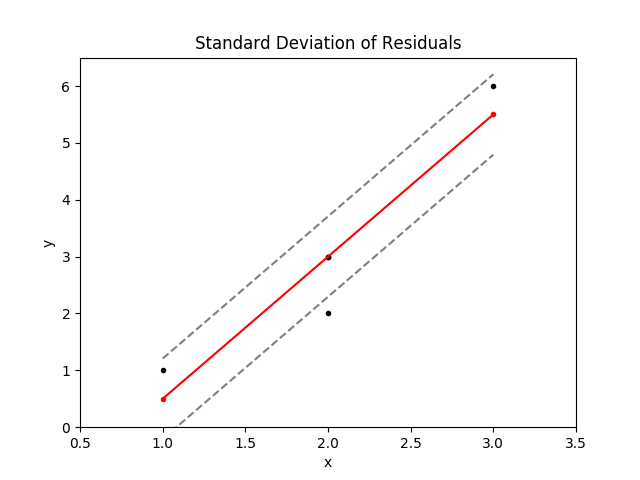
\includegraphics[scale=0.99]{standard-deviation-of-residuals}

\paragraph{Summary:}
This is used to find out how much a model disagrees with the actual data. A \textbf{lower number} means a \textbf{better} fit to the model.

% LINKS: -
% Khan Academy: https://www.khanacademy.org/math/statistics-probability/describing-relationships-quantitative-data/assessing-the-fit-in-least-squares-regression/v/standard-deviation-of-residuals-or-root-mean-square-error-rmsd
\end{document}
